\documentclass[11pt]{article}

\usepackage[margin=1in]{geometry}
\usepackage{amsmath,amssymb}
\newcommand{\Q}{\mathbb{Q}}
\usepackage{graphicx}
\usepackage{tikz}
\usetikzlibrary{arrows.meta,positioning,fit}
\usepackage{booktabs}
\usepackage{array}
\usepackage{microtype}
\setlength{\emergencystretch}{3em}
\usepackage[hidelinks]{hyperref}
\usepackage{url}

\title{Podium: An Open-Source Library for Rendezvous and\\
Docking Guidance, Navigation, and Control with\\
Integrated Formal Verification}
\author{Adi Oltean\thanks{Starcloud, Inc. Source and documentation:
\texttt{github.com/adi-oltean/podium}. Archived at
\url{https://doi.org/10.5281/zenodo.21225268}.}}
\date{July 2026}

\begin{document}
\maketitle

\begin{abstract}
Podium is an open-source Python library for developing, testing, and formally
validating guidance, navigation, and control (GNC) algorithms for spacecraft
rendezvous, proximity operations, and docking (RPOD) in low- and medium-Earth
orbit. It provides relative-motion models, convex and sequential-convex
trajectory planners, a relative-navigation filter and controllers, a
deterministic simulator, and a verification layer. The flight-algorithm core is
written in a restricted, statically analyzable Python subset that translates to
C, is shown alarm-free on contracted input ranges by the Frama-C Evolved Value
Analysis (EVA) plug-in \cite{framac2015}, a sound static analyzer, and is
compiled with the CompCert verified compiler \cite{compcert2009}, with the
emitted C checked against the Python reference on golden vectors. Several guarantees are re-verified
in exact rational arithmetic in the trusted checker: tolerance-free barrier
certificates for abort safety, Karush--Kuhn--Tucker (KKT) certificates that bound
the suboptimality of an approximate online convex solve within an explicit
rational tolerance, and tolerance-free bounds on the global optimum of the
nonconvex docking subproblem. This paper describes the architecture, the
verification approach, and a reproducible end-to-end example.
\end{abstract}

\section{Motivation and significance}

Spacecraft rendezvous and docking place strong demands on
software~\cite{fehse2003}. The maneuvers
are safety-critical, and some unsafe commands or contact events cannot be
corrected after the fact; they run convex and nonconvex optimization in the loop; and the flight code must be shown to be free
of runtime errors and faithful to its specification. Mature simulation
environments exist, including Basilisk \cite{basilisk2020}, NASA's 42
\cite{nasa42}, Orekit \cite{orekit2010}, and the General Mission Analysis Tool
(GMAT) \cite{gmat2020}, and Podium
does not attempt to replace them for general astrodynamics. Its purpose is
narrower: to organize development around spacecraft rendezvous, proximity
operations, and docking (RPOD) rather than absolute orbit propagation, and to
make formal validation part of ordinary development.

The library is motivated by three needs. Relative motion, approach corridors,
keep-out zones, plume impingement, and docking contact are central to RPOD and
are a modeling focus distinct from absolute orbit propagation. Convex trajectory
optimization is now standard in guidance
\cite{acikmese2007,acikmese2011,szmuk2018,malyuta2022}, but a
floating-point quadratic program (QP) or second-order cone program (SOCP) solver
can return a
nominally optimal solution that violates a constraint under rounding, so Podium
re-verifies each online solve with an exact-rational Karush--Kuhn--Tucker (KKT)
checker, certifying the floating-point solution within an explicit rational
optimality tolerance, before the command is used. The gap between a Python prototype and
analyzable flight-target C, ordinarily crossed by hand, is here crossed
mechanically, so that validation evidence applies to the same code path intended
for deployment.

\section{Software description}

\begin{figure}[t]
\centering
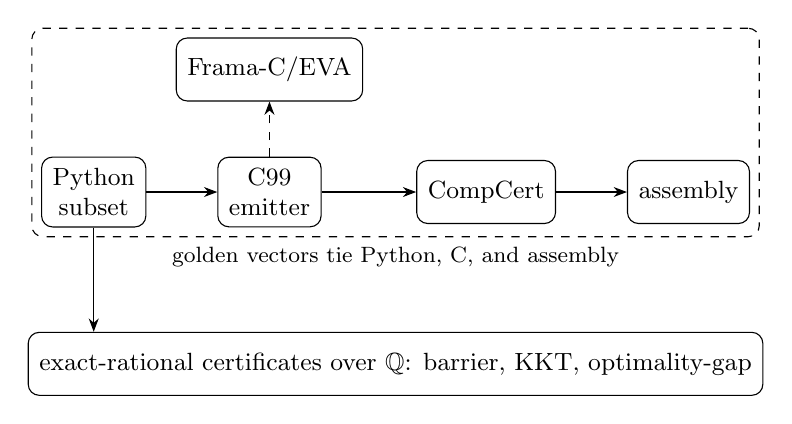
\begin{tikzpicture}[
  font=\small,
  box/.style={draw, rounded corners, align=center, inner sep=4pt,
              minimum height=8mm},
  >={Stealth[]}]
\node[box] (py) {Python\\subset};
\node[box, right=9mm of py] (emit) {C99\\emitter};
\node[box, right=12mm of emit] (cc) {CompCert};
\node[box, right=9mm of cc] (asm) {assembly};
\draw[->] (py) -- (emit);
\draw[->] (emit) -- (cc);
\draw[->] (cc) -- (asm);
\node[box, above=7mm of emit] (eva) {Frama-C/EVA};
\draw[->, dashed] (emit.north) -- (eva.south);
\node[draw, dashed, rounded corners, fit=(py)(asm)(eva),
      label=below:{\footnotesize golden vectors tie Python, C, and assembly}]
      (path) {};
\node[box, below=12mm of path.south, minimum width=88mm] (cert)
      {exact-rational certificates over $\Q$:
       barrier, KKT, optimality-gap};
\draw[->] (py.south) -- (py.south |- cert.north);
\end{tikzpicture}
\caption{The flight-code path (top): a restricted Python subset is emitted to
C99, shown alarm-free by Frama-C/EVA, and compiled by CompCert, with golden
vectors tying the Python, C, and assembly on the tested inputs. A separate layer
re-runs the exact-rational certificates (verified over $\Q$) together with
reachability checks on every change.}
\label{fig:arch}
\end{figure}

\subsection{Architecture}

Podium is organized as subpackages under \texttt{src/podium}. The \texttt{core}
package holds the verifiable algorithm core: the Clohessy--Wiltshire dynamics and
state-transition matrix \cite{clohessy1960}, the Yamanaka--Ankersen matrix for
elliptic orbits \cite{yamanaka2002}, relative orbital elements with Keplerian, $J_2$, and
$J_2$-plus-drag state-transition matrices \cite{koenig2017}, a quaternion kernel,
and fixed-step integrators. The \texttt{dynamics} package holds the truth models:
nonlinear relative motion with $J_2$ and differential drag over a seeded
stochastic atmosphere, and rigid-body attitude with a suite of environmental
torques (gravity gradient, aerodynamic, solar radiation pressure, and magnetic).

The \texttt{guidance} package implements convex and sequential-convex trajectory
planners on the relative-motion discretizations. The \texttt{control} package
provides discrete and continuous linear-quadratic regulators, quaternion attitude
feedback, and a push-only thruster allocation. The \texttt{nav} package
implements a relative-navigation extended Kalman filter with a Joseph-form
(numerically stable) covariance update and sensor models for relative
satellite navigation (relative Global Navigation Satellite System, GNSS), camera,
and lidar. The \texttt{sim} package provides a deterministic
fixed-step engine with bit-identical replays, Signal Temporal Logic (STL)
specification oracles, and contact checking. The \texttt{verify} and \texttt{emit}
packages provide the verification layer and the C code generator described below.

\subsection{A verifiable algorithm core}

Flight algorithms are written as pure step functions in a restricted subset of
Python: statically shaped arrays, bounded loops, no dynamic allocation, and
machine-readable contracts on input ranges and invariants. The subset is chosen
so that a sound static analyzer can reason about it and so that it translates
line-for-line to C. The \texttt{emit} package generates C99 from the subset,
annotated with ACSL (ANSI/ISO~C Specification Language) contracts, together with
correctly rounded implementations of the transcendental functions from CORE-MATH
\cite{coremath2022}. The Frama-C/EVA
abstract-interpretation analyzer
\cite{framac2015} shows the emitted C free of runtime alarms (division by zero,
overflow, invalid access) on the contracted input ranges. The generated C is
checked against the Python reference on a suite of golden vectors, bit-exact for
arithmetic and square root and correctly rounded for transcendentals; the same
vectors are replayed through the CompCert verified compiler \cite{compcert2009},
which machine-checks semantics preservation from C to assembly for the supported
C subset and calling convention, and on a second instruction-set architecture
(ISA) to confirm bit-identical results. The golden vectors thus tie the Python reference,
the emitted C, and the compiled assembly on the tested inputs.

\paragraph{Software metadata.}
Repository \texttt{github.com/adi-oltean/podium}; language Python 3.11+; license
MIT; principal dependencies NumPy, CVXPY, and Clarabel, with optional
verification tooling (Frama-C, CompCert, JuliaReach). Continuous integration runs
on GitHub Actions. The examples and the per-release audit bundle are the primary
distribution channel; the library is in active development (v0.x).

\section{Verification approach}

Podium runs verification as a set of automated checks re-executed on every
relevant change, rather than as a manual milestone; Table~\ref{tab:lanes}
summarizes them.

\begin{table}[t]
\centering
\caption{Automated verification checks, each re-run in continuous integration.
QP: quadratic program. SOCP: second-order cone program. QCQP: quadratically
constrained quadratic program. ISA: instruction-set architecture.}
\label{tab:lanes}
\begin{tabular}{@{}>{\raggedright\arraybackslash}p{0.34\linewidth}>{\raggedright\arraybackslash}p{0.62\linewidth}@{}}
\toprule
Check & Guarantee \\
\midrule
Closed-loop reachability (JuliaReach \cite{juliareach2019}) & flowpipes avoid unsafe sets on the benchmark models \cite{archcomp2023} \\
Exact-rational barrier certificates & infinite-horizon abort safety, verified over $\Q$ \\
Exact-rational KKT certificates & online QP and SOCP solves certified within an explicit rational optimality tolerance, checked over $\Q$ \\
Exact optimality-gap certificates & bounds on a nonconvex QCQP optimum, verified over $\Q$ \\
Sound static analysis (Frama-C/EVA) & emitted C alarm-free on contracted input ranges \\
Verified compiler and cross-ISA & golden vectors preserved through CompCert and a second ISA \\
Independent physics oracle & translational truth model cross-validated against Orekit \cite{orekit2010} \\
\bottomrule
\end{tabular}
\end{table}

Two implementation choices support these guarantees. Several certificates are
checked in exact rational arithmetic, with no floating point in the trusted
checker: a barrier for abort safety \cite{prajna2004,ames2017}, KKT conditions
for the online convex solves, and bounds on the global optimum of the nonconvex
docking subproblem through the S-procedure \cite{yakubovich1971,polik2007} and
its trust-region special case \cite{moresorensen1983}. The
barrier and optimality-gap certificates are tolerance-free, their acceptance
being an exact positive-semidefiniteness test together with exact feasibility;
exact rational certificates of this kind build on a body of work in
sum-of-squares and polynomial optimization and in verified semidefinite
programming \cite{parrilo2003,lasserre2001,kaltofen2012,peyrl2008,davis2022}.
The KKT check re-verifies an approximate solver output, so it computes the
optimality residuals exactly and accepts the point when they lie within an
explicit rational tolerance, which is then a certified bound on the point's
suboptimality. In every case the checker itself introduces no rounding error. The emitted flight C is tied to the Python reference by
bit-exact golden vectors and carried to assembly by CompCert, so the validated
algorithm and the compiled algorithm agree on the tested inputs. Every tagged
release ships an audit bundle, produced by a build script that archives the
continuous-integration receipts under a fixed seed, whose hash is reproducible
across rebuilds.

\section{Illustrative example}

Two artifacts illustrate the library at different depths. A one-command demo,
\texttt{examples/\allowbreak vbar\_approach.py}, plans a one-kilometer approach along the
target's velocity axis (a V-bar approach, in the local-vertical/local-horizontal
frame) on the Clohessy--Wiltshire discretization and propagates it under the
linear Clohessy--Wiltshire dynamics; Figure~\ref{fig:vbar} shows its trajectory.
It is a readable entry point (Python 3.11+, dependencies in
\texttt{pyproject.toml}, no other setup) and is not the verified pipeline.

The full pipeline is the reference mission (\texttt{podium.sim.mission},
exercised by \texttt{test\_mission.py} in continuous integration): a convex
planner whose online solve is re-verified by the exact-rational KKT checker,
which certifies the floating-point solution within an explicit rational
optimality tolerance; propagation through the nonlinear truth model with $J_2$
and differential drag; checking of the closed-loop trajectory against
approach-corridor and keep-out Signal Temporal Logic specifications; and
certification of the passive-drift abort safety (the safe free-drift trajectory
after a thruster cutoff) by the exact barrier. An interactive playback of the
approach is hosted at \url{https://adi-oltean.github.io/podium/} as static HTML
with no build step, and the emitted flight kernels are exercised in
\texttt{examples/cfs\_nav\_app/}, a NASA Core Flight System (cFS) application,
with build and run steps in its \texttt{README}.

\begin{figure}[t]
\centering
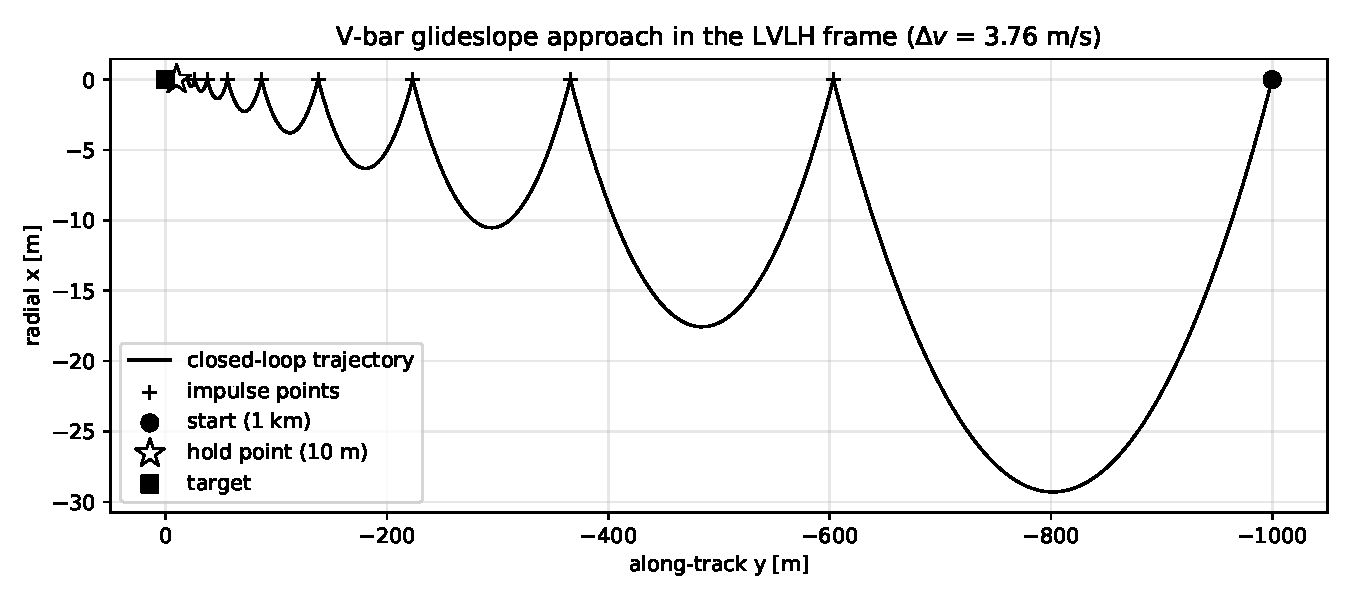
\includegraphics[width=0.86\linewidth]{vbar.pdf}
\caption{Trajectory of the \texttt{vbar\_approach.py} demo: a one-kilometer V-bar
glideslope approach to a 10\,m hold point in the local-vertical/local-horizontal
(LVLH) frame, planned on the Clohessy--Wiltshire discretization and propagated
under the linear Clohessy--Wiltshire dynamics. The verified pipeline (KKT
certification, nonlinear truth model, and barrier) is the reference mission,
exercised in continuous integration rather than by this demo.}
\label{fig:vbar}
\end{figure}

\section{Impact and comparison}

Each ingredient of Podium is well covered by open prior art; the contribution is
their coupling. Table~\ref{tab:compare} makes this precise against the closest
tools on each axis.

\begin{table}[t]
\centering
\caption{Podium's claim is a conjunction: each open tool covers at most one or
two prongs. \checkmark{} full, $\sim$ partial, blank none. Prong (i): a
sequential-convex planner; (ii): exact-rational per-solve certificates re-run in
continuous integration; (iii): a restricted high-level-source-to-C path checked
by golden vectors, Frama-C/EVA, and CompCert. RPOD marks a rendezvous/docking
focus.}
\label{tab:compare}
\begin{tabular}{@{}lcccc@{}}
\toprule
& (i) SCP & (ii) cert/CI & (iii) verified C & RPOD \\
\midrule
SCPToolbox.jl \cite{scptoolbox2022}                 & \checkmark & & $\sim$ & $\sim$ \\
GuSTO.jl \cite{gusto2019}                           & \checkmark & &        & $\sim$ \\
ct-scvx \cite{elango2025}                           & \checkmark & & $\sim$ & $\sim$ \\
successive\_rendezvous \cite{successive_rendezvous2020} & \checkmark & &    & \checkmark \\
RealCertify \cite{magron2018}                       & & $\sim$ & & \\
ValidSDP \cite{validsdp}                            & & $\sim$ & & \\
Verified SDP \cite{jansson2009}                     & & $\sim$ & & \\
Copilot \cite{copilot2023}                          & & & \checkmark & \\
Credible autocoding \cite{feron2013,cohen2020}      & $\sim$ & & $\sim$ & \\
{CVXPYgen} \cite{cvxpygen2022}                      & & & $\sim$ & \\
Basilisk \cite{basilisk2020}                        & & & & \checkmark \\
\textbf{Podium}                                     & \checkmark & \checkmark & \checkmark & \checkmark \\
\bottomrule
\end{tabular}
\end{table}

On trajectory optimization, the open SCPToolbox.jl \cite{scptoolbox2022} and
GuSTO.jl \cite{gusto2019} implement the sequential-convex family with
rendezvous and free-flyer examples, ct-scvx \cite{elango2025} adds continuous-time
feasibility with in-house C generation, and successive\_rendezvous
\cite{successive_rendezvous2020} is a released 6-DoF Apollo transposition-and-docking
implementation; prong (i) for RPOD is thus established open art, and none of these
carries a certificate or verified-code layer. On certificates, RealCertify
\cite{magron2018}, the Coq-checked ValidSDP \cite{validsdp}, and verified SDP
\cite{jansson2009} produce exact-rational or rigorously bounded certificates for
general polynomial and conic problems, but not online, not RPOD-specific, and not
re-run in continuous integration. On verified code, the Copilot toolchain
\cite{copilot2023} couples a restricted high-level source with a C path, formal
proof, and CI (for runtime monitors, not guidance); credible autocoding
\cite{feron2013,cohen2020} autocodes convex-optimization solvers to
contract-annotated C; and CVXPYgen \cite{cvxpygen2022} generates C from Python
convex problems, none with exact-rational certificates. The simulators Basilisk
\cite{basilisk2020} and NASA's 42 \cite{nasa42} and the flight-dynamics systems
Orekit \cite{orekit2010} and GMAT \cite{gmat2020} support proximity-operations
modeling but no planner, certificate, or verified-code layer.

The novelty is therefore not any single prong but their integration. We are not
aware of a publicly released, RPOD-focused library that, in one codebase, couples
sequential-convex planners with exact-rational \emph{per-solve} certificates
re-run in continuous integration and a restricted Python-to-C flight-code path
whose generated C is regression-checked by golden vectors, analyzed by
Frama-C/EVA under stated input contracts, and compiled by CompCert over its
supported subset. Podium is complementary to the tools above rather than a
replacement. It is intended for researchers and engineers developing and
validating RPOD guidance and control, and as a reproducible baseline: verification
runs on every change and every release carries its evidence, so that results built
on the library can be re-checked independently.

\section{Conclusions}

Podium is an open library that organizes guidance, navigation, and control around
RPOD scenarios from the outset and treats formal validation as a continuous
activity. Its verifiable algorithm core, exact-arithmetic certificates, and
verified flight-code path are designed so that validation evidence applies to the
same code path intended for deployment, and so that its guarantees can be
reproduced by any user. The exact-rational certificates are checked by an
$O(n^3)$ symmetric $LDL^\top$ factorization, whose factors are themselves the
nonnegativity witness; the open problem is to scale this from the per-primitive
matrices to the block-banded matrices of a full trajectory, where a fraction-free
elimination exploiting the bandedness would bound the certificate size in the
horizon. Development continues toward broader mission coverage and such
structure-exploiting exact certificates.

\bibliographystyle{unsrt}
\bibliography{references}

\end{document}
